\documentclass[a4paper]{article}

\usepackage{caption}
\usepackage{listings}
\usepackage{fancyhdr}
\usepackage[top=3cm,bottom=3cm,left=3cm,right=3cm]{geometry}
\usepackage{color}
\usepackage{amsmath}
\usepackage{graphicx}

\definecolor{dkgreen}{rgb}{0,0.6,0}
\definecolor{gray}{rgb}{0.5,0.5,0.5}
\definecolor{mauve}{rgb}{0.58,0,0.82}

\lstset{frame=tb,
  language=Octave,
  aboveskip=3mm,
  belowskip=3mm,
  showstringspaces=false,
  columns=flexible,
  basicstyle={\small\ttfamily},
  numbers=none,
  numberstyle=\tiny\color{gray},
  keywordstyle=\color{blue},
  commentstyle=\color{dkgreen},
  stringstyle=\color{mauve},
  breaklines=true,
  breakatwhitespace=true,
  tabsize=3
}

\newcommand{\HRule}{\rule{\linewidth}{0.5mm}}
\pagestyle{fancy}
\lfoot{\small \color{gray}Tom Peerdeman - 10266186}
\cfoot{\thepage}
\rfoot{\small \color{gray}Ren\'e Aparicio Sa\'ez - 10214054}
\lhead{\small \color{gray}Autonome Mobiele Robots}

\begin{document}
\begin{titlepage}
\begin{center}
\textsc{\Large Autonome Mobiele Robots}\\[0.5cm]
\HRule \\[0,4cm]
\textsc{\huge \bfseries NXT - Steering}
\HRule \\[8cm]
\begin{minipage}{0.4\textwidth}
\begin{flushleft}\large
\emph{Auteurs: Tom Peerdeman \& Ren\'e Aparicio Saez}\\
\end{flushleft}
\end{minipage}
\begin{minipage}{0.4\textwidth}
\begin{flushright}\large
\emph{Datum: \today\\\hspace{1cm}}\\
\end{flushright}
\end{minipage}
\end{center}
\end{titlepage}

\section{Materiaal}
Om de experimenten uit dit rapport te kunnen uitvoeren zijn de volgende materialen gebruikt:\\
- PC/Laptop met Matlab\\
- Boek: Autonomous Mobile Robots 2th Edition - Roland Siegwart et al.
- NXT-Robot\\
- Pen en papier
\section{Kinematica}
\begin{figure}[h]
	\centering
	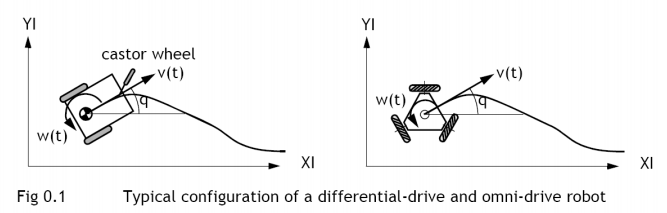
\includegraphics[width=0.8\textwidth]{imgs/robots.png}
	\label{fig:lineairverband}
\end{figure}
\subsection{Kinematica van twee robots}
Robot met twee wielen:\\
$\mathrm{[\dot{x}\; \dot{y}\; \dot{\theta}]^T} = f\mathrm{(l, r, \theta, \dot{\varphi_{1}}, \dot{\varphi_{2}})}$\\
\\
De variabelen voor het castor-wiel hoeven niet meegenomen te worden in de functie, omdat het castor-wiel niet gemotoriseerd is. Omdat deze daarom geen invloed uitoefent op de richting of snelheid van het voertuig, kan het castor-wiel gezien worden als een sleepwiel dat in de functie te verwaarlozen valt.\\\\
Robot met drie wielen:\\
$\mathrm{[\dot{x}\; \dot{y}\; \dot{\theta}]^T} = f\mathrm{(l, r, \theta, \dot{\varphi_{1}}, \dot{\varphi_{2}}, \dot{\varphi_{3}})}$\\


\subsubsection{Odometry}
a.De makkelijkste manier om te kijken naar de invloed van de draaisnelheiden van de wielen op de positie en de orientatie is door deze eerst te bepalen in het robot co\"ordinaten stelsel. Dit is makkelijker te bepalen aangezien de robot in dit co\"ordinaten stelsel nooit een snelheid kan krijgen in de y richting door de constraint dat er geen slip aanwezig is.\\
De snelheid in de x richting is ook makkelijk te bepalen. Stel dat alleen wiel 1 draait met snelheid $\dot{\varphi_{1}}$, aangezien P in het midden ligt van wiel 1 en 2 zal deze zich dus voorbewegen met een snelheid van $\frac{1}{2}r\dot{\varphi_{1}}$ in de x richting. Aangezien dit ook geldt als alleen wiel 2 draait kunnen we deze optellen als allebei de wielen draaien.
In het geval dat de wielen draaien met snelheden $\dot{\varphi_{1}}$ en $\dot{\varphi_{2}}$ zal de robot dus een snelheid krijgen van $\frac{1}{2}r\dot{\varphi_{1}} + \frac{1}{2}r\dot{\varphi_{2}}$ in de x richting.\\\\
De rotatie is op een zelfde manier te berekenen. stel dat wiel 1 stil staat en wiel 2 zo draait dat er een positieve snelheid in de x richting ontstaat. In dit geval gaat de robot draaien om het contactpunt van wiel 1. We kunnen zeggen dat wiel 2 rijd op een circkel met radius 2l en als middelpunt het contactpunt van wiel 1. Aangezien we de draaisnelheid weten van wiel 2 kunnen we de rotatiesnelheid van dit wiel berekenen met de volgende formule:\\
$\omega_{1}=\frac{r\dot{\varphi_{1}}}{2l}$\\
Stel nu dat wiel 1 draait en wiel 2 stilstaat, we krijgen dan ook een rotatie, echter in de andere richting dan eerst.
De formule blijft dus hetzelfde op het feit na dat de draairichting, en dus de rotatiesnelheid negatief wordt:
$\omega_{2}=-\frac{r\dot{\varphi_{2}}}{2l}$\\
Aangezien de rotatiesnelheid in situatie 1 in het punt P gelijk is aan dat van wiel 2, en in situatie 2 die van wiel 1 kunnen we deze optellen om zo de totale rotatiesnelheid te krijgen in punt P: $\omega=\frac{r\dot{\varphi_{1}}}{2l}-\frac{r\dot{\varphi_{2}}}{2l}$\\\\
We weten nu alle benodigde snelheden in robot co\"ordinaten:\\\\
$
\dot{\xi_{R}}
\begin{bmatrix}
\frac{1}{2}r\dot{\varphi_{1}} + \frac{1}{2}r\dot{\varphi_{2}} \\
0\\
\frac{r\dot{\varphi_{1}}}{2l}-\frac{r\dot{\varphi_{2}}}{2l}
\end{bmatrix}
=
\begin{bmatrix}
\dot{x} \\
\dot{y} \\
\dot{\theta}
\end{bmatrix}_{R}
$
\\\\
We kunnen nu de snelheden omzetten naar wereld co\"ordinaten door de inverse van de rotatiematrix te gebruiken:\\
$
\dot{\xi_{I}}=
R(\theta)^{-1}
\begin{bmatrix}
\frac{1}{2}r\dot{\varphi_{1}} + \frac{1}{2}r\dot{\varphi_{2}} \\
0\\
\frac{r\dot{\varphi_{1}}}{2l}-\frac{r\dot{\varphi_{2}}}{2l}
\end{bmatrix}
=
R(-\theta)
\begin{bmatrix}
\frac{1}{2}r\dot{\varphi_{1}} + \frac{1}{2}r\dot{\varphi_{2}} \\
0\\
\frac{r\dot{\varphi_{1}}}{2l}-\frac{r\dot{\varphi_{2}}}{2l}
\end{bmatrix}
$
\\\\\\
b. 1. De precisie van de inschatting verbetert naarmate de $\Delta t$ afneemt. Dit komt omdat als de positie net geschat is en de robot zich beweegt, de positie voor een tijd van $\Delta t$ incorrect is. Als $\Delta t$ afneemt zal de precisie van de gemiddelde inschatting dus toenemen.\\\\
2. De rotatie snelheid in robot co\"ordinaten is uitgewerkt in opgave a. Aangzien de rotatiematrix echter niks doet met deze waarde is deze waarde dus gelijk aan de rotatiesnelheid in het wereldco\"ordinaten stelsel. De rotatiesnelheid is dus:\\
$w(t) = \omega=\frac{r\dot{\varphi_{1}}}{2l}-\frac{r\dot{\varphi_{2}}}{2l}$\\\\
3. De v vector heeft twee elementen: de snelheid in de x richting en de snelheid in de y richting. We kunnen de v vector dus berekenen door de x en y snelheid in robot co\"ordinaten te vermenigvuldigen met een niet homogene rotatiematrix over de hoek $-\theta$:\\\\
$
\vec{v}=
\begin{bmatrix}
\dot{x} \\
\dot{y}
\end{bmatrix}
=
\begin{bmatrix}
cos(-\theta) & sin(-\theta)\\
-sin(-\theta) & cos(-\theta)
\end{bmatrix}
\begin{bmatrix}
\frac{1}{2}r\dot{\varphi_{1}} + \frac{1}{2}r\dot{\varphi_{2}} \\
0
\end{bmatrix}
$

\section{Steering Experimenten}

\subsection{Theorie (a)}
De robot moet onderscheidt kunnen maken tussen twee basis bewegingen. Een rechte lijn en een bocht maken (deel van de vorm van een cirkel).\\
\\
De theorie voor een rechte lijn rijden is eenvoudig. De robot moet weten wat de af te leggen afstand $\psi$ is en met welke snelheid $\varphi$ hij deze moet gaan afleggen. Als deze waarden bekend zijn, kan bepaald worden hoeveel tijd de wielen dit moeten uitvoeren en kan een rechte lijn gereden worden.\\
\\
Een bocht maken is wat minder eenvoudig. Hiervoor moet bekend zijn wat de afstand van elk wiel tot aan het middelpunt van de robot is $l$ (deze afstand is voor elk gemotoriseerd wiel hetzelfde). Daarnaast moet bekend zijn wat de radius $r$ van de cirkel is waar omheen gereden moet worden. Deze radius wordt bepaald vanaf het middelpunt $P$ van de robot tot aan het middelpunt van de cirkel die de bocht definieert. Er moet ook bekend zijn hoeveel graden $\alpha$ er moet worden gedraaid. De snelheid voor de wielen moet vervolgens per wiel berekend worden. De snelheid $\varphi_1$ voor het wiel aan de buitenkant van de bocht wordt geleverd. Om de snelheid voor het tweede wiel te bepalen moet eerst bepaald worden wat de afstand is die elk wiel moet afleggen. Dit wordt als volgt bepaald:\\\\
voor het wiel aan de buitenkant van de bocht:
$s_1 = \frac{2\pi(r + l)}{360}\alpha$\\
voor het wiel aan de binnenkant van de bocht:
$s_2 = \frac{2\pi(r - l)}{360}\alpha$\\\\
Vervolgens kan de tijd $t$ bepaald worden door de afstand voor het buitenste wiel te delen door de meegeleverde bijbehorende snelheid. Deze berekende $t$ geeft aan hoelang het wiel moet draaien. Als $t$ bekend is kan ook de snelheid voor het binnenste wiel worden berekend. $\varphi_2=\frac{s_2}{t}$

\subsection{Feedback  (b)}
Als bewegingen zijn uitgevoerd kan nagegaan worden of dit juist is verlopen. Door tijdens het uitvoeren van een beweging bij te houden of de wielen de juiste afstand hebben afgelegd kan bepaald worden of er afgeweken is van de oorspronkelijke waarde. Als deze waarde afwijkt van de oorspronkelijke waarde moet hiervoor gecompensserd worden bij de volgende beweging. Dit kan worden gedaan door de afstand die teveel of te weinig is afgelegd, van de volgende beweging af te halen.

\subsection{Implementatie zonder kinematica}
\subsubsection{Rechte lijn}
De implementatie voor de rechte lijn is vrij voor de hand liggend. Beide wielen krijgen dezelfde power mee. De afstand wordt in cm meegegeven. Deze moet vervolgens worden omgerekend naar het aantal graden dat de wielen moeten draaien. Hiervoor is de omtrek van de gemotoriseerde wielen nodig. Dit kan berekend worden omdat de diameter bekend is, deze is namelijk 5.6cm. De omtrek wordt dan $\pi * 5.6 = 17.593cm$. Het aantal omwentelingen kan vervolgens worden bepaald door de te rijden afstand te delen door deze omtrek en te vermenigvuldigen met 360 graden.
\begin{lstlisting}[caption=Rechte lijn, label=lst:line, numbers=left]
function NXTLine(phi, afstand)
wentels = afstand/17.593 * 360;
NXT_SetOutputState(MOTOR_B, phi, true, true, 'SPEED', 0, 'RUNNING', wentels, 'dontreply');
NXT_SetOutputState(MOTOR_C, phi, true, true, 'SPEED', 0, 'RUNNING', wentels, 'dontreply');
\end{lstlisting}
\subsubsection{Bocht}
Voor de bocht moeten er meerdere berekeningen gedaan worden. De theorie blijft van kracht, er vormt zich echter een probleem voor de tijdseenheid. De snelheid die meegegeven wordt aan de functie, is niet het aantal rotaties/toeren per minuut maar de power die de motor levert. Echter blijkt dat het verband tussen de power ten opzichte van het aantal toeren per minuut lineair is. (Zie figuur \ref{fig:lineairverband}) Dit betekent dat de vreemde snelheids eenheid, namelijk de power, geen invloed heeft op het berekenen van de tijd. De tijd wordt echter van de waarde afstand per power. Omdat continu met dezelfde eenheden wordt gewerkt wordt uiteindelijk de eenheid voor de snelheid van het tweede wiel gewoon power. Vervolgens wordt de afstand die afgelegd moet worden omgerekend naar het aantal graden dat elk wiel moet draaien, zodat dit aan de call kan worden meegegeven. Tenslotte moet er bekeken worden welke kant opgedraaid moet worden, links of rechts. Aan de hand van een if else statement kan hier op worden gecontroleerd.
\begin{figure}[h]
	\centering
	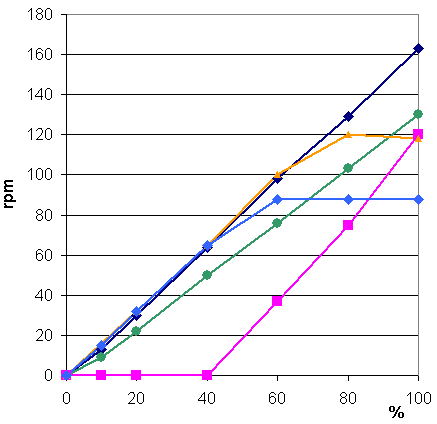
\includegraphics[width=0.6\textwidth]{imgs/lineair.png}
	\caption{Lineair verband, donkerblauw is voor een ongeladen motor, 9V NXT motor\protect\footnotemark}
	\label{fig:lineairverband}
\end{figure}
\footnotetext{Original source: http://www.philohome.com/nxtmotor/nxtmotor.htm}
\\\\
\vspace{5cm}
\begin{lstlisting}[caption=Bocht, label=lst:bocht, numbers=left]
function NXTBocht(radius, alpha, phi1, richting)
s1 = (2*pi*(radius+5.85))/360 * alpha;
s2 = (2*pi*(radius-5.85))/360 * alpha;
t = s1 / phi1;
phi2 = s2/t;
wentel1 = s1/17.593 * 360;
wentel2 = s2/17.593 * 360;
% bocht naar rechts
if richting
NXT_SetOutputState(MOTOR_C, phi1, true, true, 'SPEED', 0, 'RUNNING', wentel1, 'dontreply');
NXT_SetOutputState(MOTOR_B, phi2, true, true, 'SPEED', 0, 'RUNNING', wentel2, 'dontreply');
% bocht naar links
else
NXT_SetOutputState(MOTOR_C, phi2, true, true, 'SPEED', 0, 'RUNNING', wentel2, 'dontreply');
NXT_SetOutputState(MOTOR_B, phi1, true, true, 'SPEED', 0, 'RUNNING', wentel1, 'dontreply');
end
\end{lstlisting}
\subsubsection{Meerdere bewegingen}
Tot slot moet er voor gezorgd worden dat er meerdere bewegingen achter elkaar kunnen worden uitgevoerd. Hiervoor moet per beweging worden gewacht totdat deze klaar is. Hier wordt op gecheckt door de status van de motors te bekijken. Zodra deze geen power meer leveren wordt het signaal 'IDLE' afgegeven. Zodra dit signaal is ontvangen kan een eventueel volgende beweging worden uitgevoerd.
\\\\
\begin{lstlisting}[caption=Meerdere moves, label=lst:moves, numbers=left]
while(1)
    outB = NXT_GetOutputState(MOTOR_B);
    outC = NXT_GetOutputState(MOTOR_C);
    if strcmp(outB.RunStateName, 'IDLE') && strcmp(outC.RunStateName, 'IDLE')
        break
    end
end
\end{lstlisting}
\subsubsection{Feedback}
Error compensatie bij rechte lijnen lijkt erg vanzelfsprekend. Er wordt bekeken hoeveel graden de motor voor de omwenteling heeft gemaakt voor de beweging, en hoeveel omwentelingen er gedaan zijn na de beweging. Het verschil tussen deze twee waarden zou gelijk moeten zijn aan de oorspronkelijk ingevoerde waarde voor de omwentelingen. Het verschil hiertussen is de error. Om zeker te weten dat er geen error compensatie wordt uitgevoerd van bewegingen uit een oud programma, moet deze worden geinitialisserd bij het starten van de bewegingen. 
\begin{lstlisting}[caption=Error compensatie bij een lijn, label=lst:lineerror, numbers=left]
function NXTLinet(phi, wentels)
global error
outB = NXT_GetOutputState(MOTOR_B);
beforeB = outB.TachoCount;
outC = NXT_GetOutputState(MOTOR_C);
beforeC = outC.TachoCount;
NXT_SetOutputState(MOTOR_B, phi, true, true, 'SPEED', 0, 'RUNNING', wentels-error(1), 'dontreply');
NXT_SetOutputState(MOTOR_C, phi, true, true, 'SPEED', 0, 'RUNNING', wentels-error(2), 'dontreply');
while(1)
    outB = NXT_GetOutputState(MOTOR_B);
    outC = NXT_GetOutputState(MOTOR_C);
    if strcmp(outB.RunStateName, 'IDLE') && strcmp(outC.RunStateName, 'IDLE')
        break
    end
end

outB = NXT_GetOutputState(MOTOR_B);
afterB = outB.TachoCount;
outC = NXT_GetOutputState(MOTOR_C);
afterC = outC.TachoCount;
diffB = abs(afterB-beforeB)+error(1);
diffC = abs(afterC-beforeC)+error(2);
error = [diffB-wentels diffC-wentels];

\end{lstlisting}
Uit experimenten blijkt echter dat de berekende error-waarden erg fluctueren. Bij dezelfde gereden afstand met dezelfde snelheid verschilt de error tussen 20 en 60 graden (gemeten door de TachoCount). Er is dus geen verband tussen afstand en error te vinden, of tussen snelheid en error. Zonder te compenseren voor deze error-waarden worden betere resultaten bereikt. Dus is besloten voor de bocht geen error-compensatie door middel van TachoCount te maken.

\subsection{Implementatie met Kinematica}
\subsubsection{Open loop}
Als er gebruik gemaat moet worden van kinematica moet de code verder worden aangepast. Er hoeven minder waarden aan de functie meegegeven te worden. Als de radius van de te maken bocht en de hoek waarover gedraaid moet gaan worden in radialen bekend zijn, kunnen alle overige waarden berekent worden. Bij een rechte lijn zijn de radius en de te maken hoek nul, er is dan geen kinematica nodig. Aan de hand van de meegegeven radius en de te rijden hoek alpha kan een onderlinge snelheidsverhouding voor de wielen worden bepaald. Dit wordt gedaan door gebruik te maken van inverse kinematica. De standaard formule om een nieuwe locatie van de robot te bepalen is:\\\\
$
\begin{bmatrix}
\dot{x}\\
\dot{y}\\
\dot{\theta}
\end{bmatrix}=
\begin{bmatrix}
cos(\theta) & -sin(\theta) & 0\\
sin(\theta) & cos(\theta) & 0\\
0 & 0 & 1\\
\end{bmatrix}
\begin{bmatrix}
\frac{r}{2} & \frac{r}{2} & 0\\
0 & 0 & 1\\
\frac{r}{2l} & \frac{r}{2l} & 0\\
\end{bmatrix}
\begin{bmatrix}
\dot{\varphi_{1}}\\
\dot{\varphi_{2}} 
\end{bmatrix}
$\\\\
Hieruit willen we $\dot{\varphi_{1}}$ en $\dot{\varphi_{2}}$ halen. Hiervoor moet de formule worden omgeschreven. De nieuwe formule wordt dan:\\\\
$
\begin{bmatrix}
\dot{\varphi_{1}}\\
\dot{\varphi_{2}} 
\end{bmatrix}
=
\begin{bmatrix}
\frac{r}{2} & \frac{r}{2} & 0\\
0 & 0 & 1\\
\frac{r}{2l} & \frac{r}{2l} & 0\\
\end{bmatrix}^{-1}
\begin{bmatrix}
cos(\theta) & sin(\theta) & 0\\
-sin(\theta) & cos(\theta) & 0\\
0 & 0 & 1\\
\end{bmatrix}
\begin{bmatrix}
\dot{x}\\
\dot{y}\\
\dot{\theta}
\end{bmatrix}
$\\\\
Hierbij is $\dot{x} = r*sin(\theta)$ en $\dot{y} = r-r*cos(\theta)$ als er naar rechts wordt gedraaid en $\dot{y} = r+r*cos(\theta)$ als er naar links wordt gedraaid. $\dot{\theta}$ is gelijk aan de te maken draaihoek in radialen. Als $r$ en $l$ ook bekend zijn kunnen $\varphi_1$ en $\varphi_2$ berekent worden. De waarden voor phi geven het aantal totaal te maken omwentelingen aan per wiel in radialen. 
Uit de te maken omwentelingen kan een snelheid bepaald worden. Omdat het aantal omwentelingen in verhouding van elkaar staan, kan door middel van een aangegeven maximale power de onderlinge power van de wielen worden bepaald. Bijvoorbeeld:\\\\
$\dot{\varphi_{1}} = 10$\\
$\dot{\varphi_{2}} = 8$\\
$power_{max} = 40$\\\\
$if (\dot{\varphi_{1}} > \dot{\varphi_{2}})\ \{$\\
$power_1 = power_{max}$\\
$power_2 = \frac{\dot{\varphi_{2}}}{\dot{\varphi_{1}}}power_{max}$\\
$\}\ else\ \{$\\
$power_1 = \frac{\dot{\varphi_{1}}}{\dot{\varphi_{2}}}power_{max}$\\
$power_2 = power_{max}$\\
$\}$
\subsubsection{Feedback}
In het boek van Siegwart et al. wordt een manier geopperd om de robot zijn fouten te laten corrigeren. Hiervoor wordt gebruik gemaakt van de volgende formule:\\\\
$
\begin{bmatrix}
\dot{\rho}\\
\dot{\alpha}\\
\dot{\beta}
\end{bmatrix}
=
\begin{bmatrix}
-k_{\rho}\rho cos(\alpha)\\
k_{\rho}sin(\alpha)-k_{\alpha}\alpha-k_{\beta}\beta\\
-k_{\rho}sin(\alpha)
\end{bmatrix}
=
\begin{bmatrix}
- cos(\alpha) & 0 \\
\frac{sin(\alpha)}{\rho} & -1\\
-\frac{sin(\alpha)}{\rho} & 0
\end{bmatrix}
\begin{bmatrix}
v \\
\omega
\end{bmatrix}
$
\\\\
waarbij:\\\\
$\rho = \sqrt{\Delta x^2 + \Delta y^2}$\\
$\alpha = -\psi+ atan2(\Delta y, \Delta x)$\\
$\beta = \theta - atan2(\Delta y, \Delta x)$\\
$v = k_{\rho}\rho$\\
$\omega = k_{\alpha}\alpha  + k_{\beta}\beta$\\\\
Hierbij zijn $\Delta x$ en $\Delta y$ de afstanden in de $x$ en $y$ richting die de robot heeft afgelegd in een van te voren aangegeven interval $\Delta t$. $\theta$ is de hoek die totaal gedraaid moet worden vanaf begin tot eind en $\psi$ is de hoek die gedraaid is vanaf het begin tot het huidige moment . $k_{\rho}$, $k_{\alpha}$ en $k_{\beta}$ zijn drie variabelen die gekozen kunnen worden en bepalen hoe de robot wordt bijgestuurd als hij van zijn baan raakt.\\
Zodra de robot dichter bij de eindlocatie komt, zullen $\rho$, $\alpha$ en $\beta$ richting $0$ gedrongen worden. Het is echter vrijwel onmogelijk om exact op $0$ uit te komen. Daarom moet gebruik gemaakt worden van een variantie. Er wordt een error vector bepaald, die bekijkt wat de te bereieken locatie is en wat de huidige locatie is. Door deze twee waarden te vergelijken met elkaar kan bekeken worden hoe dicht de robot bij zijn eindpunt is. Als deze error vector waarden binnen de aangegeven variantie liggen, is de eindlocatie zo goed als bereikt. Als de waarden niet binnen de variantie vallen moet doorgereden worden. Met behulp van de te berekenen $v$ en $\omega$ kan weer door middel van inverse kinematica bepaald worden wat de snelheden per wiel zijn. Als vervolgens een aangegeven tijdinterval $\Delta t$ voorbij is, kan opnieuw de error vector bepaald gaan worden, net zo lang totdat ze waarden binnen de variantie hebben bereikt.

\subsubsection{Resultaten \& uiteindelijke code}
Als een lage $\Delta t$ gekozen wordt zal het programma het beste werken. Bij een te hoge $\Delta t$ zal de robot kunnen doorschieten. Bij het plotten van de data komt er met een $\Delta t$ van $0.01s$ een mooie bocht uit (zie figuur: \ref{fig:goed}). Bij een $\Delta t$ van $1s$ schiet de robot te ver door en zal hij zichzelf oneindig proberen te corrigeren (zie figuur: \ref{fig:slecht}).\\
Bij een lage variantie zal de robot zo exact mogelijk naar het einddoel proberen toe te rijden. Als de variante te laag is zal de robot nooit het doel bereiken en doorschieten, om zichzelf vervolgens te corrigeren (zie figuur: \ref{fig:lowvar}).

\begin{lstlisting}[caption= Kinematica met feedback code, label=lst:bocht, numbers=left]
function MoveWithFeedBack(dx, dy, do, maxpower, r, l, kp, ka, kb, dt)
% Cumulative position in world coordinates
posx = 0;
posy = 0;
post = 0;

% Variance, at dest if the value is between var_ and -var_
varx = 0.5;
vary = 0.2;
vart = pi/10.0;

% Reset initial motor position to 0 rotations
NXT_ResetMotorPosition(MOTOR_B, false);
NXT_ResetMotorPosition(MOTOR_C, false);

while 1
    m1 = NXT_GetOutputState(MOTOR_B);
    m2 = NXT_GetOutputState(MOTOR_C);
    
    % phi1 en phi2 over a period of dt time
	v1 = (m1.RotationCount / 180 * pi) / dt
	v2 = (m2.RotationCount / 180 * pi) / dt
	
    NXT_ResetMotorPosition(MOTOR_B, false);
    NXT_ResetMotorPosition(MOTOR_C, false);
	
    % Get the speed we rotated with in dt time
	dott = GetThetaSpeed(v1, v2, r, l);
	
    % Get the speed in x and y using our current rotation
	[dotx, doty] = GetSpeed(v1, v2, post, r)
    
    % Update the current rotation
	post = post + (dott * dt);
	
    % Calculate our x and y pos since the start of this movement
	posx = posx + (dotx * dt);
	posy = posy + (doty * dt);

	error = [dx - posx; dy - posy; do - post]
    
    % error is approx at 0, we are at the destination
	if error(1) >= -varx && error(1) <= varx && error(2) >= -vary && error(2) <= vary && error(3) >= -vart && error(3) <= vart
		break;
	end
	
   
    rho = sqrt(error(1)^2 + error(2)^2);
	
    lambda = atan2(error(2), error(1));
	alpha = modangle(lambda - post);
	beta = modangle(do - lambda);
    
	v = kp * rho;
	rotationspeed = ka * alpha + kb * beta;
	
	[phi1, phi2] = InvKinematics(v, 0, rotationspeed, post, r, l);
	
    % Calculate the power, it is linair to the wheel rotation speed
	[p1, p2] = GetPower(phi1, phi2, maxpower);

	NXT_SetOutputState(MOTOR_B, p1, true, true, 'SPEED', 0, 'RUNNING',  0, 'dontreply');
	NXT_SetOutputState(MOTOR_C, p2, true, true, 'SPEED', 0, 'RUNNING',  0, 'dontreply');
	
	pause(dt);
end

% Stop motors
NXT_SetOutputState(MOTOR_B, 0, true, false, 'IDLE', 0, 'RUNNING',  0, 'dontreply');
NXT_SetOutputState(MOTOR_C, 0, true, false, 'IDLE', 0, 'RUNNING',  0, 'dontreply');

% Transform an angle to make sure it is in [-pi, pi]
function [a] = modangle(angle)
a = mod(angle, 2*pi);
if a > pi
    a = a - (2 * pi);
end

% Transform wheel rotation speeds to power
function [p1, p2] = GetPower(phi1, phi2, maxpower)
d = phi1/phi2;
% Wheel 1 turns fastest and thus should have power = maxpower
if phi1 > phi2
	p1 = maxpower;
	p2 = phi2/phi1 * maxpower;
else
    % Wheel 2 turns fastest and thus should have power = maxpower
	p1 = phi1/phi2 * maxpower;
	p2 = maxpower;
end

function [speedt] = GetThetaSpeed(phi1, phi2, r, l)
speedt = r/(2*l) * phi1 - r/(2*l) * phi2;

function [speedx, speedy] = GetSpeed(phi1, phi2, omega, r)
% Xi_I = R(omega)-1*Xi_R*[phi1; phi2]
Rinv = [cos(omega) -sin(omega); sin(omega) cos(omega)];
XI_R = [1/2*r*phi1 1/2*r*phi2; 0 0;];

XI_I = Rinv * XI_R;

speedx = XI_I(1);
speedy = XI_I(2);
function [phi1, phi2] = InvKinematics(speedx, speedy, speedtTheta, theta, r, l)
% Xi_I = R(omega)-1*Xi_R*[phi1; phi2]
% R(omega) * Xi_I = Xi_R*[phi1; phi2]
% Xi_R-1 * R(omega) * Xi_I = [phi1; phi2]
XI_R = [1/2*r 1/2*r 0; 0 0 1; r/(2*l) -r/(2*l) 0];
R = [cos(theta) sin(theta) 0; -sin(theta) cos(theta) 0; 0 0 1];

phiVect = inv(XI_R) * R * [speedx; speedy; speedtTheta];
phi1 = phiVect(1);
phi2 = phiVect(2);
\end{lstlisting}

\begin{figure}[h]
	\centering
	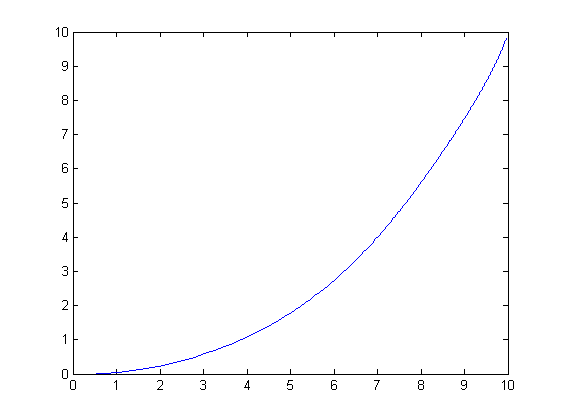
\includegraphics[width=0.7\textwidth]{imgs/example_plot.png}
	\caption{Plot voor de call: MoveWithFeedBackPlot(10, 10, pi/2, -1, 5.6, 5.8, 3, 8, -1.5, 0.01)}
	\label{fig:goed}
\end{figure}
\begin{figure}[h]
	\centering
	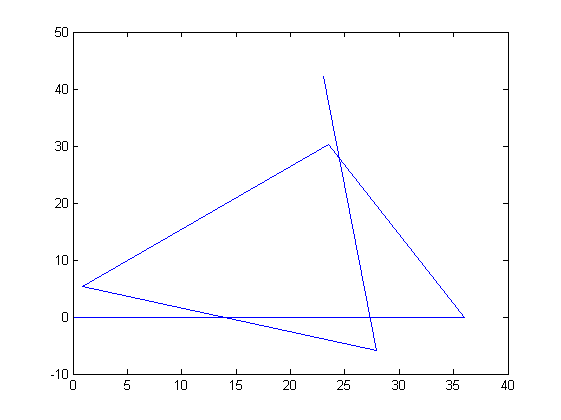
\includegraphics[width=0.7\textwidth]{imgs/fail_dt.png}
	\caption{Plot voor de call: MoveWithFeedBackPlot(10, 10, pi/2, -1, 5.6, 5.8, 3, 8, -1.5, 1)}
	\label{fig:slecht}
\end{figure}
\begin{figure}[h]
	\centering
	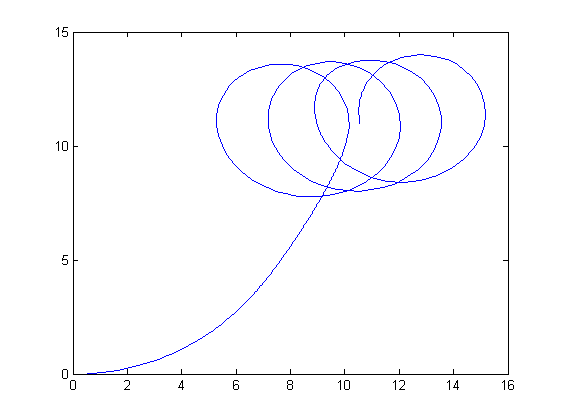
\includegraphics[width=0.7\textwidth]{imgs/small_variance.png}
	\caption{Plot met variantie varx = 0.1; vary = 0.1; vart = pi/20.0; en $\Delta t = 0.01$}
	\label{fig:lowvar}
\end{figure}
\end{document}
